%%
%% Kapitel
%%
\chapter{Einsatz von Sprachmodellen}
Im Zuge dieser Arbeit wurden Versuche mit verschiedenen Sprachmodellen durchgef\"uhrt, die im Folgenden beschrieben werden.

\section{Versuchsaufbau}
Der Source Code f\"ur die Versuche ist in Python verfasst, da die Sprachmodelle alle eine \"ubersichtliche Schnittstelle zur Verwendung in Python bieten. Die erstellten Netze sind durch die Bibliotheken \textit{keras} \cite{keras} und \textit{Tensorflow} \cite{tensorflow} implementiert worden. \\
Der Code wurde zum Testen in \textbf{Jupyter Notebooks} auf Googles Plattform \textit{Google Colab} \cite{colab} ausgef\"uhrt, da mit dieser Plattform eine Laufzeitumgebung mit M\"oglichkeit zur Nutzung von einer GPU sowie - falls n\"otig - einer TPU zur Verf\"ugung steht. Die genaue Spezifikation der GPU kann dabei nicht ausgew\"ahlt werden, es sind \textit{Nvidia K80s, T4s, P4s} und \textit{P100s} verf\"ugbar \cite{colab_gpu}. Die genutzten Datens\"atze werden \"uber Links zu der Datenquelle (\textit{kaggle.com, github.com}) oder lokal eingebunden.

Als Vergleichswerte zwischen den Sprachmodellen wurden die Genauigkeiten bei der Auswertung der jeweiligen Datens\"atze sowie die \textbf{F1-score} hergenommen. Der \textbf{F1-Wert} berechnet sich wie in Gleichung 3.1 beschrieben, wobei \textit{tp} f\"ur \textit{true positives}, \textit{fp} f\"ur \textit{false positives} und \textit{tp} f\"ur \textit{true negatives} stehen.
\begin{align}
   F1 {=} \frac{tp}{tp + \frac{1}{2} \dot (fp + fn)}
\end{align}
Die Zeit zum Ausf\"uhren wurde gemessen, gibt aber aufgrund der unterschiedlichen genutzten GPUs keine hohe Aussagekraft sondern gibt blo{\ss} einen ungef\"ahren Richtwert bei Nutzung einer GPU.

\subsection{Verwendete Bibliotheken}
F\"ur die verschiedenen Sprachmodelle ist die Nutzung mehrer Bibliotheken f\"ur python n\"otig. Diese werden in dem jeweiligen Notebook eingebunden und teilweise zur Laufzeit installiert. Diese Bibliotheken sindim Folgenden aufgestellt:
\begin{itemize}
\item \textbf{Tensorflow}
\item \textbf{Fastai}
\item \textbf{Torch}
\item \textbf{gpt}
\item \textbf{simpletransformers} \cite{simpletransformers} f\"ur die Einbindung der transformerbasierten Sprachmodelle
\item \textbf{sklearn} f\"ur Auswertung der Ergebnisse
\item \textbf{nltk, pandas, string} und andere Standardbibliotheken f\"ur Textverarbeitung 
\end{itemize}

\section{Die Daten}
F\"ur \textbf{Sentiment Analysis} werden ausschlie{\ss}lich Daten genutzt, die von der Plattform \textit{Twitter} genommen wurden. Diese Daten eignen sich sehr gut f\"ur diese Aufgabe, da die L\"ange der Textst\"ucke auf 280 Zeichen begrenzt ist \cite{twitter} und es eine gro{\ss}e Nutzerbasis und damit eine gro{\ss}e Vielfalt an formulierten Texten gibt. Hierbei werden die Tweets genommen, die nur Text und entsprechende Emojis enthalten und in Englisch verfasst sind. Die genutzten Datens\"atze sind gelabelt, um damit \textbf{Supervised Learning} zu betreiben, da die Feinabstimmung der Sprachmodelle so erfolgen muss.\\
Die Daten werden alle vorverarbeitet, um die Texte einheitlich und gut verarbeitbar zu machen. Hierzu werden f\"ur die Tweets folgende Schritte durchgangen:
\begin{itemize}
\item alle W\"orter in Kleinbuchstaben umwandeln
\item doppelte Buchstaben entfernen (aus "`helloooo"' wird z.B. "`hello"') 
\item Whitespaces an Anfang und Ende entfernen
\item Emojis entfernen
\end{itemize}
Die Daten f\"ur den Teil \textbf{Stance detection} haben unterschiedliche Urspr\"unge. Datens\"atze bestehen haupts\"achlich aus Artikeln, deren \"Uberschriften und den jeweiligen angesprochenen Stances. Auch diese Daten werden einer Datenreinigung unterzogen. Diese unterscheidet sich nur leicht von der f\"ur die \textbf{Sentiment Analysis} durchgef\"uhrte, da die Artikel im Allgemeinen keine sogenannten \textit{handles} oder Emojis enthalten. Diese Datens\"atze sind gelabelt, um einen sp\"ateren Test m\"oglich zu machen.\\
Wie bei sehr vielen Machine Learning Aufgaben h\"angen die Ergebnisse stark von der Qualit\"at der genutzten Daten ab. Es wurde demnach versucht, alle Datens\"atze so zu reinigen, dass die Performanz optimal wurde. Auf etwaige zus\"atzliche Schritte wird in der jeweiligen Beschreibung eingegangen.\\
Die Datens\"atze werden in Test- und Trainingsdaten aufgeteilt, wobei der Anteil der Testdaten 33\% des gesamten Datensatzes ist.

%subsections für die verschiedenen Datensätze 

\subsection{Apple Sentiment}
\label{sec:applesent}
Dieser Datensatz ist manuell gelabelt und wurde urspr\"unglich von \textit{crowdflower} \cite{crowdflower} zur Verf\"ugung gestellt. Die 1630 englischsprachigen Tweets wurden aufgrund von \textit{hashtags} gefiltert, die die Firma \textit{Apple} betreffen. Die hier verwendete Version \cite{apple_sent} ist soweit gefiltert, dass nur Tweets und Labels enthalten sind. Alle nicht relevanten Tweets wurden ebenfalls entfernt. Die Labels dieses Datensatzes sind -1 (negativ), 0 (neutral) und 1 (positiv).\\
\lstset{language=Python}
\lstset{frame=lines}
\lstset{caption={S\"auberung des Datensatzes}}
\lstset{captionpos=b}
\lstset{label={lst:clean_140}}
\lstset{basicstyle=\footnotesize}
\begin{lstlisting}
df_train.tweet = df_train.tweet.str.lower()
df_test.tweet = df_test.tweet.str.lower()

# Delete URLs
df_train.text = df_train.text.apply(lambda x:re.sub(r'http\S+', '', x))
df_test.text = df_test.text.apply(lambda x:re.sub(r'http\S+', '', x))

#Tokenize, better for emojis, double characters and handle stripping than pure text
tokenizer = TweetTokenizer(strip_handles=True, reduce_len=True)
df_train.tweet = df_train.tweet.apply(lambda x: tokenizer.tokenize(x))
df_test.tweet = df_test.tweet.apply(lambda x: tokenizer.tokenize(x))

# Detokenize for better processing
df_train.tweet = df_train.tweet.apply(lambda x: ' '.join(x))
df_test.tweet = df_test.tweet.apply(lambda x: ' '.join(x))

df_train.tweet = df_train.tweet.map(lambda x : 
	x.translate(str.maketrans('', '', string.punctuation)))
df_test.tweet = df_test.tweet.map(lambda x : 
	x.translate(str.maketrans('', '', string.punctuation)))

df_train.tweet = df_train.tweet.str.replace("[0-9]", " ")
df_test.tweet = df_test.tweet.str.replace("[0-9]", " ")

df_train.tweet = df_train.tweet.str.strip(string.whitespace)
df_test.tweet = df_test.tweet.str.strip(string.whitespace)

# Recreate index that was shuffeled when splitting test and train
df_train = df_train.reset_index(drop=True)
df_test = df_test.reset_index(drop=True)
\end{lstlisting}
In diesem Datensatz sind keine Emojis enthalten, die entfernt werden m\"ussten. Die S\"auberung erfolgt wie in Listing \ref{lst:clean_140} dargestellt und das Ergebnis ist in folgender Tabelle dargestellt:

%Beispiele aus gesäubertem Datensatz
\begin{center}
\begin{tabular}{|c|c|}
\hline
tweet & sentiment\\ 
\hline\hline
the secret of life from steve jobs in    seconds& \\ some motivation from the late ceo of&0\\
\hline
it took just one month for the iphone plus& \\to become the king of phablets  is king  jobspring technews&1\\
\hline
imessage isnt working thanks&-1\\
\hline    
\end{tabular}
\end{center}


\subsection{US Airline Sentiment}
\label{sec:airlinesent}
Wie auch der Datensatz aus Teil \ref{sec:applesent} wurde der \textbf{US Airline Sentiment} durch Anwendung von Filtern von \textit{Twitter} bezogen \cite{airlines}. Der Datensatz besteht aus 14640 in Englisch verfassten Tweets mit manuell gelabelten Meinungen der Nutzer zu verschiedenen Fluggesellschaften. Die Einteilung der Sentiment-Werte ist hier als Label statt numerisch gegeben: Es gibt die Labels \textit{neutral, negative} und \textit{positive}. Zur Verarbeitung durch die Sprachmodelle wurden diese Labels jeweils numerisch codiert.\\
Da in den Texten noch Emojis vorhanden sind, werden diese durch den in Listing \ref{lst:clean_airline} gezeigten Code entfernt. Es wurden ebenfalls Versuche mit noch enthaltenen Emojis durchgef\"uhrt. Beispiele aus dem ges\"auberten Datensatz sind in der folgenden Tabelle gegeben.
%Code zur Säuberung
\lstset{language=Python}
\lstset{frame=lines}
\lstset{caption={Funktion zum Entfernen von Emojis}}
\lstset{captionpos=b}
\lstset{label={lst:clean_airline}}
\lstset{basicstyle=\footnotesize}
\begin{lstlisting}
def remove_emoji(string):
    emoji_pattern = re.compile("["
                           u"\U0001F600-\U0001F64F"  # emoticons
                           u"\U0001F300-\U0001F5FF"  # symbols & pictographs
                           u"\U0001F680-\U0001F6FF"  # transport & map symbols
                           u"\U0001F1E0-\U0001F1FF"  # flags (iOS)
                           u"\U00002702-\U000027B0"
                           u"\U000024C2-\U0001F251"
                           "]+", flags=re.UNICODE)
    return emoji_pattern.sub(r'', string)
\end{lstlisting}
%Beispiele aus gesäubertem Datensatz
\begin{center}
\begin{tabular}{|c|c|}
\hline
tweet & sentiment\\ 
\hline\hline
youre my early frontrunner for best airline  oscars&positive\\
\hline
what is going on with your bdl to dca flights yesterday&\\ and today   why is every single one getting delayed&negative\\
\hline
do they have to depart from washington  d  c&neutral\\
\hline    
\end{tabular}
\end{center}

\subsection{T4SA}
\label{sec:t4sa}
Der \textbf{T4SA} Datensatz \cite{t4sa} wurde von seinen Entwicklern zur \textbf{Cross-Media-Analyse} genutzt. Hierbei wurden zun\"achst die Texte der Tweets nach sentiment-Werten klassifiziert, um die ebenfalls in den Tweets enthaltenen Bilder zu labeln. Auch diese Tweets wurden gefiltert um sicherzustellen, dass alle Tweets Bilder enthalten, in Englisch verfasst und mindestens f\"unf W\"orter lang sind. In dieser Arbeit stehen die enthaltenen Bilder nicht zur Betrachtung, aber der zu Sentiment-Werten gelabelte Datensatz l\"asst sich gut verwenden.\\
Hier genutzt werden 1179957 der im Datensatz enthaltenen Tweets. Diese Teilmenge besteht nur aus mit Sentiment-Werten versehenen Tweets. Da die Daten auf mehrere Dateien verteilt sind, ist eine etwas aufwendigere Vorverarbeitung notwendig: Zus\"atzlich zu der in Listing \ref{lst:clean_140} und \ref{lst:clean_airline} aufgef\"uhrten Testverarbeitung werden die beiden Dateien in einen Dataframe zusammengefasst, indem die Tweet-ID jeweils als Schl\"usselwert genommen wird. Die Sentiment-Werte liegen in der Original-Datei als in drei Spalten (\textit{POS, NEG} und \textit{NEU}) aufgeteilte Wahrscheinlichkeitswerte vor. Der Spaltenname mit der h\"ochsten eingetragenen Wahrscheinlichkeit wird im Folgenden als das Label der Zeile genommen und in den Modellen entsprechend numerisch codiert. Beispiele aus dem final genutzten Dataframe sind in der folgenden Tabelle aufgef\"uhrt.
%Beispiele aus gesäubertem Datensatz
\begin{center}
\begin{tabular}{|c|c|}
\hline
tweet & sentiment\\ 
\hline\hline
inbound marketing content ideas part&NEU\\
\hline
i think this song is about phil im excited&POS\\
\hline
yo this the ugliest filter eveeer son  im weaaak&NEG\\
\hline    
\end{tabular}
\end{center}

\subsection{Fake News Challenge}
\label{sec:tfnc}
Dieser Datensatz besteht aus 49972 Artikeln, verschiedenen Aussagen, die \"uber den Text (oder einen anderen) getroffen wurden und der Beziehung zwischen den Aussagen und den Artikeln \cite{fnc}. Beziehungen werden in die Kategorien "`unrelated"', "`agree"', "`discuss"' und "`disagree"' eingeordnet. Diese Klassifizierung wurde f\"ur die Verarbeitung durch die Modelle numerisch codiert. Der Inhalt ist unbalanciert, 73\% der Trainingsdaten sind mit "`unrelated"', 18\% mit "`discuss"' und die restlichen 9\% mit "`disagree"' oder "`agree"' gelabelt. Da es sich hier um Artikel handelt, m\"ussen bei der Datenreinigung keine Emojis oder \textit{Twitter-Handles} beachtet werden. Die in unterschiedlichen Dateien vorliegenden Artikel werden den Aussagen zugeordnet und danach in Kleinbuchstaben umgewandelt. Zeichensetzung sowie Whitespaces an Anfang und Ende des Artikels werden entfernt. Gek\"urzte Beispiele aus dem Datensatz sind im Folgenden gelistet.
%Beispiele aus gesäubertem Datensatz
\begin{center}
\begin{tabular}{|c|c|c|}
\hline
Aussage & Artikel & Stance\\ 
\hline\hline
 mexico says students not& more graves have been discovered at  & discuss\\
 among dead in mass grave & the site where 43 students went missing &\\
\hline
isis beheads american & afghanistan veteran sam arnold uploaded this & unrelated\\
 photojournalist james wright & spinechilling  video of a us marine getting &\\
 foley threatens more to come & a direct headshot from a taliban sniper [...] &\\
\hline    
\end{tabular}
\end{center}

\subsection{SemEval}
\label{sec:semeval}
\textbf{SemEval} wurde urspr\"unglich f\"ur einen ausgeschriebenen Wettbewerb erstellt \cite{semeval}. In diesem Datensatz sind 2056 Tweets enthalten, die gegen drei unterschiedliche \textbf{Targets} auf ihre Haltung \"uberpr\"uft wurden. Die Haltung ist klassifiziert durch die Kategorien "`AGAINST"', "`FAVOR"' und "`NONE"'. Auch hier wurden die Kategorien numerisch codiert. Die S\"auberung l\"auft analof zu der S\"auberung der Tweets in den vorangegangenen Datens\"atzen. Die Themen dieses Wettbewerbs sind Hillary Clinton, Donald Trump, Atheismus, Feminismus, Klimawandel ist real und das Recht auf Abtreibung.

%Beispiele aus gesäubertem Datensatz
\begin{center}
\begin{tabular}{|c|c|c|}
\hline
Target & Tweet & Stance\\ 
\hline\hline
 hillary clinton & and  handovertheserver she wiped clean  30k deleted & AGAINST\\
  & emails  explains dereliction of duty  lies re benghazi  etc tcot semst  &\\
\hline
hillary clinton & hillary is our best choice if we truly want to & FAVOR\\
&  continue being a progressive nation  ohio semst &\\
\hline    
\end{tabular}
\end{center}

\section{Sentiment Analysis}
Im Folgenden werden die Experimente zu \textbf{Sentiment Analysis} im Detail beschrieben. Hierbei wird zun\"achst das verwendete Modell beschrieben und dann auf die spezifischen Aspekte wie Codierung der Labels und Ergebnisse zu den verschiedenen Datens\"atze eingegangen. 

\subsection{Ausgangsbasis}
Um einen Vergleich zu haben, wie performant und genau \textbf{Sentiment Analysis} mit Sprachmodellen ist, wurde zun\"achst ein Ansatz ausgewertet, der keinen Gebrauch von Deep Learning macht. Die Ver\"anderung der Genauigkeit im Vergleich zu diesem Ansatz gibt einen Anhaltspunkt, wie viel Sprachmodelle in Sentiment Analysis leisten k\"onnen.\\
Der jeweilige Datensatz wird mit pythons \textit{pandas} Bibliothek eingelesen, ges\"aubert und im Anschluss mit der Bibliothek \textit{TextBlob} ausgewertet. Diese Auswertung basiert auf manuell erstellten Dokumenten, in denen allen W\"ortern Sentiment-Werte zugeordnet wurden. \textit{TextBlob} werten diese Werte f\"ur einen gegebenen Text aus und gibt einen Wert zwischen -1 und 1 zur\"uck (negativ zu positiv). Um mit den Labels der Datents\"atze vergleichbar zu sein, wurden diese float-Werte zur jeweils n\"achsten ganzen Zahl gerundet. Da diese Auswertung sequentiell erfolgt, wurde keine GPU genutzt. Die Auswertung erfolgt durch den in Listing \ref{lst:code_direct} aufgezeigten Code. Um besser vergleichbar zu sein, wurde, wie in den anderen Modellen jeweils nur der Test-Dataframe ausgewertet.
%Code zu TextBlob
\lstset{language=Python}
\lstset{frame=lines}
\lstset{caption={Auswertung mit TextBlob}}
\lstset{captionpos=b}
\lstset{label={lst:code_direct}}
\lstset{basicstyle=\footnotesize}
\begin{lstlisting}
data.insert(2, "blobpolarity", 
	data.text.map(lambda x: int(round(TextBlob(x).sentiment.polarity)), 
	True)
\end{lstlisting}

\subsubsection*{Apple Sentiment}
Die Einstufungen m\"ussen bei diesem Datensatz nicht umgerechnet werden. Aufgrund der begrenzten Anzahl an Daten in dem Datensatz dauert die Berechnung der Sentiment-Werte unter einer Minute. Der Genauigkeitswert liegt bei 53,0\%.

\subsubsection*{US Airline Sentiment}
In diesem Datensatz werden die Labels in eine numerische Form gebracht, sodass die Werte analog zum letzten Experiment bei -1, 0 und 1 liegen. Auch bei diesem Datensatz dauert die Auswertung unter einer Minute. Es wird eine Genauigkeit von 25,7\% erreicht.

\subsubsection*{T4SA}
Wie in dem \textbf{US Airline Sentiment} Datensatz werden die Labels numerisch codiert. Die Auswertung dauert 3 Minuten und ergibt eine Genauigkeit von 66,1\%.

\subsubsection*{Auswertung}
Die Genauigkeitswerte schwanken stark, da kein Lernvorgang stattfindet und alle Datens\"atze nach dem gleichen Prinzip ausgewertet werden, obwohl sie an sich unterschiedliche Sprachaspekte enthalten. Die h\"aufigste Klassifizierung von TextBlob ist "`Neutral"', wodurch die \textbf{F1-Score} hier meist am h\"ochsten ist. Die Datens\"atze sind dabei nicht ganz ausgeglichen und in den Tests\"atzen \textbf{Apple Sentiment} und \textbf{T4SA} sind mehr neutral klassifizierte Tweets enthalten, was sich in der h\"oheren Genauigkeit niederschl\"agt.
\begin{center}
\begin{tabular}{|c||c|c|c|}
\hline
F1 score & Apple Sentiment & US Airline Sentiment & T4SA\\ 
\hline\hline
-1 & 0,156 & 0,098 & 0,185\\
\hline
0 & 0,675 & 0,349 & 0,758\\ 
\hline
1 & 0,286 & 0,283 & 0,543\\
\hline    
\end{tabular}
\end{center}

%ELMo
\subsection{ELMo}
Die verwendeten Datens\"atze werden zun\"achst ges\"aubert und in einen Dataframe eingelesen. Daraufhin wird das ELMo-Modell geladen und die Vektoren f\"ur die Eingabe bestimmt: Hierbei wird f\"ur eine Eingabesequenz ein einziger Vektor durch Mittelwertbildung bestimmt, um eine gute Weiterverarbeitung zu garantieren. Diese 1024-dimensionalen Vektoren werden abgespeichert, um immer auf sie zugreifen zu k\"onnen.\\
Da ELMo kein eigenes Modell zur Sentiment Analysis bietet, werden hier zwei verschiedene Ans\"atze erprobt:
\begin{itemize}
\item Logistic Regression
\item einschichtiges LSTM-Netz
\end{itemize}
Bei der \textbf{Logistischen Regression} wird eine Funktion gesucht, die die Beziehung zwischen den \textbf{ELMo}-Vektoren und den Labels des Datensatzes modelliert.\\
Das einschichtige LSTM-Netz wurde mithilfe von \textit{keras} implementiert, der Input ist der 1024-dimensionale Wortverktor. Dieser wird in eine LSTM-Schicht mit 512 Neuronen gegeben, um danach in einer \textbf{fully connected} Schicht weiterverarbeitet und zu einem drei Labels umfassenden Output gemappt, wie Listing \ref{lst:elmo_lstm_model} zeigt. Die Anzahl der zu trainierenden Epochen wurde anhand des \textbf{Validation Loss} bestimmt.
\lstset{language=Python}
\lstset{frame=lines}
\lstset{caption={Aufbau des LSTM-Netzes}}
\lstset{captionpos=b}
\lstset{label={lst:elmo_lstm_model}}
\lstset{basicstyle=\footnotesize}
\begin{lstlisting}
_________________________________________________________________
Layer (type)                 Output Shape              Param #   
=================================================================
lstm_1 (LSTM)                (None, 512)               3147776   
_________________________________________________________________
dense_1 (Dense)              (None, 3)                 1539      
_________________________________________________________________
activation_1 (Activation)    (None, 3)                 0         
=================================================================
\end{lstlisting}

\subsubsection*{Apple Sentiment}
Die Bestimmung der Wortvektoren dauert ca. 15 Sekunden, die Auswertung erfolgt in unter einer Sekunde. Mit der \textbf{Logistischen Regression} wird eine Genauigkeit von 83,8\% erreicht. Das LSTM-Netz wird in 20 Epochen trainiert und liefert eine Genauigkeit von 82,0\%.

\subsubsection*{US Airline Sentiment}
\textbf{ELMo} Wortvektoren sind nach 45 Sekunden berechnet, die Berechnung der \textbf{Logistischen Regression} dauert eine halbe Minute. Dadurch wird eine Genauigkeit von 81,0\% erreicht.  Aus dem wieder in 20 Epochen trainierten LSTM-Netz folgt eine Genauigkeit von 81,5\%.

\subsubsection*{T4SA}
Die L\"ange des Datensatzes wirkt sich in einer l\"angeren Berechnungszeit aus: Die Wortvektoren sind nach 40 Minuten bestimmt. Auch die Berechnung der \textbf{Logistischen Regression} dauert mit ... etwas l\"anger und das in ... Epochen trainierte LSTM-Modell braucht .... Die erreichten Genauigkeiten liegen bei ... bzw. .... %Probleme mit RAM

\subsubsection*{Auswertung}
Die erreichten Genauigkeiten wie auch die \textbf{F1}-Werte weisen darauf hin, dass bei der Arbeit mit \textbf{ELMo}-Vektoren der Einsatz von \textbf{Logistischer Regression} ausreichend ist, um ein Modell zu bestimmen, ein LSTM-Netz gibt kaum Verbesserungen. Die in diesem Experiment errechneten Genauigkeiten sind weit von state-of-the-art-Ergebnissen entfernt.\\
\textbf{Logistische Regression}
\begin{center}
\begin{tabular}{|c||c|c|c|}
\hline
F1 score & Apple Sentiment & US Airline Sentiment & T4SA\\ 
\hline\hline
-1 & 0,857 & 0,884 & \\
\hline
0 & 0,862 & 0,632 & \\ 
\hline
1 & 0,5 & 0,730 & \\
\hline    
\end{tabular}
\end{center}

\textbf{LSTM-Netz}
\begin{center}
\begin{tabular}{|c||c|c|c|c|}
\hline
F1 score & Apple Sentiment & US Airline Sentiment & T4SA\\ 
\hline\hline
-1 & 0,843 & 0,887 & \\
\hline
0 & 0,845 & 0,642 & \\ 
\hline
1 & 0,419 & 0,728 & \\
\hline    
\end{tabular}
\end{center}

%ULMFit
\subsection{ULMFit}
Dieses Modell wurde nach dem Beispiel in \cite{ulm_model} implementiert. Zun\"achst werden die Textdaten importiert und gereinigt. Dabei wird f\"ur alle Datens\"atze au{\ss}er \textbf{Sentiment140} eine \textbf{one-hot-Codierung} ausgef\"uhrt, da mit dem Modell Multi-Label Klassifizierung sonst nicht m\"oglich ist. Dies resultiert in drei neuen Spalten in den Dataframes (negativ, neutral und positiv), die jeweils bin\"ar codiert sind.\\

\lstset{language=Python}
\lstset{frame=lines}
\lstset{caption={Laden des ULMFit Modells}}
\lstset{captionpos=b}
\lstset{label={lst:load_ulm_train}}
\lstset{basicstyle=\footnotesize}
\begin{lstlisting}
learn = language_model_learner(data_lm, drop_mult=0.7, 
		arch = AWD_LSTM, pretrained = True)
\end{lstlisting}

Daraufhin wird das geladene \textbf{ULMFit} Sprachmodell mit den Tweet-Texten der Trainingsdaten initialisiert und verschiedene Lernraten mittels eines Lernratenfinders ausprobiert. Wie der Grafik \ref{fig:lr_ulmfit} zu entnehmen ist, ist die gew\"ahlte Lernrate 0,01.
\begin{figure}[!ht]
\centering
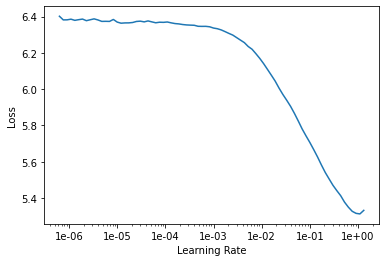
\includegraphics[height=5cm]{pics/lr_finder_ulmfit.png}
\caption{Lernratenfinder}
\label{fig:lr_ulmfit}
\end{figure}
Der n\"achste Schritt besteht aus dem \textbf{unfreezing} der Gewichte und dem Trainieren des Sprachmodells mit den Textdaten. Dazu wird die Anzahl der Epochen an den jeweiligen Datensatz angepasst. Es wird eine Anzahl gew\"ahlt, die der Gr\"o{\ss}e des Datensatzes angemessen ist und nach dem \textbf{Validation Loss} entschieden, wann gestoppt wird: Die maximale Anzahl der Epochen ist erreicht, sobald das \textbf{Validation Loss} h\"oher wird um \textbf{Overfitting} zu vermeiden. Die daraus errechneten Gewichte werden f\"ur die sp\"atere Verwendung abgespeichert.\\
Danach wird der \textbf{Classifier} trainiert. Dieser erh\"alt als Input die Textdaten und die drei Spalten f\"ur die Labels und wird nach den Metriken \textit{Genauigkeit, precision} und \textit{recall} trainiert.Mit \textbf{gradual unfreezing} werden zun\"achst nur die letzten zwei Schichten des Modellsangepasst und im n\"achsten Schritt noch einmal alle Schichten trainiert. Dieser Vorgang kann dem Listing \ref{lst:code_clas_ulm_train} entnommen werden.
\lstset{language=Python}
\lstset{frame=lines}
\lstset{caption={Gradual Unfreezing zum Trainieren des Classifiers}}
\lstset{captionpos=b}
\lstset{label={lst:code_clas_ulm_train}}
\lstset{basicstyle=\footnotesize}
\begin{lstlisting}
learn.freeze_to(-2)
learn.fit_one_cycle(2, slice(1e-2/(2.6**4),1e-2), moms=(0.8,0.7), wd=0.1)

learn.unfreeze()
learn.fit_one_cycle(2, slice(1e-3/(2.6**4),1e-3), moms=(0.8,0.7), wd=0.1)
\end{lstlisting}

\subsubsection*{Apple Sentiment}
Auch bei diesem Modell dauert das Trainieren des Modells in 20 Epochen und des Classifiers mit dem Datensatz unter einer Minute. Mit einer GPU kann hier schon ein gewisser Grad an Parallelisierung stattfinden.  Erreichte Genauigkeiten liegen bei 82,4\%. 


\subsubsection*{US Airline Sentiment}
Durch die \textbf{one-hot-Codierung} des Datensatzes f\"allt die anderweitige numerische Codierung der Labels weg. Die ermittelte Anzahl an Epochen, die das Sprachmodell trainiert wird, liegt bei zehn. Damit dauert das Training des Sprachmodells 50 Sekunden. Die Feinabstimmung des Classifiers dauert eine weitere Minute, es werden Genauigkeiten bis 88,5\% erreicht.

\subsubsection*{T4SA}
Die Vorverarbeitung verl\"auft analog zu der des \textbf{US Airline Sentiment} Datensatzes. Das Sprachmodell wird aufgrund der Menge der Daten 10 Epochen trainiert, die Trainingsdauer liegt damit bei ca 90 Minuten. Die Feinabstimmung des Classifiers dauert weitere 90 Minuten und die Genauigkeit liegt am Ende bei 97,5\%. Dieser Datensatz w\"urde von l\"angerem Training noch einen gro{\ss}en Nutzen ziehen: Nach den vergangegen Epochen war noch ein starker sinkender Trend im \textbf{Validation Loss}  zu erkennen. Dies kann mit der Gr\"o{\ss}e des Datensatzes zusammenh\"angen, da kaum M\"oglichkeiten zum \textbf{Overfitting} bestehen.

\subsubsection*{Auswertung}
Hier kann sehr gut beobachtet werden, wie sich die Gr\"o{\ss} des Datensatzes auf die Ergebnisse auswirkt: Die steigende Genauigkeit und \textbf{F1-Scores} zeigen, dass das Modell daran insgesamt besser trainieren kann. Die Gefahr des \textbf{Overfitting} ist ebenfalls sehr gering und das Modell k\"onnte insgesamt l\"anger als hier angegeben trainiert werden.
\begin{center}
\begin{tabular}{|c||c|c|c|}
\hline
F1 score & Apple Sentiment & US Airline Sentiment & T4SA\\ 
\hline\hline
-1 & 0,743 & 0,896 & 0,957\\
\hline
0 & 0,783 & 0,670 & 0,986\\ 
\hline
1 & 0,25 & 0,756 &  0,981\\
\hline    
\end{tabular}
\end{center}

%RoBERTa
\subsection{RoBERTa}
F\"ur dieses Sprachmodell m\"ussen die Eingabedaten leicht angepasst werden: Die Labels werden in die Zahlen 0, 1 und 2 codiert, damit von dem Modell verarbeitet werden k\"onnen. F\"ur die in Text gegebenen Label wird dies mit einem \textit{dictionary} gl\"ost:
\lstset{language=Python}
\lstset{frame=lines}
\lstset{caption={Umkodieren der sentiment-Label}}
\lstset{captionpos=b}
\lstset{label={lst:dict_conv_sentiment}}
\lstset{basicstyle=\footnotesize}
\begin{lstlisting}
thisdict =	{
  "negative": 0,
  "neutral": 1,
  "positive": 2
}
df_train.sentiment = df_train.sentiment.apply(lambda x: thisdict[x])
df_test.sentiment = df_test.sentiment.apply(lambda x: thisdict[x])
\end{lstlisting}
Daraufhin wird das vortrainierte Modell von \textit{pytorch} geladen und auf Multi-Label-Erkennung konfiguriert.
\lstset{language=Python}
\lstset{frame=lines}
\lstset{caption={Laden und Konfigurieren des RoBERTa-Modells}}
\lstset{captionpos=b}
\lstset{label={lst:load_config_roberta}}
\lstset{basicstyle=\footnotesize}
\begin{lstlisting}
config = RobertaConfig.from_pretrained('roberta-base')
# Set number of output labels
config.num_labels = 3
\end{lstlisting}
Die Eingabetexte werden danach in \textbf{CUDA}-Vektoren umgewandelt, um von der Parallelisierung durch GPUs Gebrauch zu machen. Das Modell wird im n\"achsten Schritt \"uber 10 Epochen mit einer Lernrate von $1^{-5}$ und dem \textbf{Adam-Optimizer} trainiert. Andere Lernraten wurden ausprobiert, gaben aber schlechtere Ergebnisse.\\
Eine alternative Version wurde mithilfe der \textbf{SimpleTransformers} Bibliothek implementiert. Diese hat den Vorteil, dass sie einfach zu nutzen und \"ubersichtlich ist, wie aus Listing \ref{lst:simple_roberta} hervorgeht.
\lstset{language=Python}
\lstset{frame=lines}
\lstset{caption={RoBERTa mit SimpleTransformers}}
\lstset{captionpos=b}
\lstset{label={lst:simple_roberta}}
\lstset{basicstyle=\footnotesize}
\begin{lstlisting}
from simpletransformers.classification import ClassificationModel

model = ClassificationModel('roberta', 'roberta-base', num_labels=3, args={
    'learning_rate':3e-5,
    'num_train_epochs': 10,
    'reprocess_input_data': True,
    'overwrite_output_dir': True,
    'process_count': 10,
    'train_batch_size': 4,
    'eval_batch_size': 4,
    'max_seq_length': 512,
    'fp16': True
})

model.train_model(df_train)
\end{lstlisting}

\subsubsection*{Apple Sentiment}
Das Training \"uber zehn Epochen mit diesem Datensatz dauert eine halbe Stunde. Weniger Epochen f\"uhren dazu, dass der Classifier nur zwischen zwei Klassen unterscheiden kann und die dritte au{\ss}er Acht l\"asst, mit mehr Epochen steigt die Gefahr des \textbf{Overfitting}. Die erreichte Genauigkeit liegt bei 78,6\%, da die dritte Klasse nur selten erkannt wird.\\
Mit dem \textbf{SimpleTransformer} Modell dauert das Training mit zehn Epochen 15 Minuten und ergibt eine Genauigkeit von 88,7\%. Auch hier wird die dritte Klasse erst nach einigen Epochen Training erkannt.

\subsubsection*{US Airline Sentiment}

\subsubsection*{T4SA}

\subsubsection*{Auswertung}
Das \textbf{RoBERTa}-Modell kann mit Multi-Klassenl Umgebungen nicht gut umgehen. Dies kann man besonders gut an den \textbf{F1}-Werten f\"ur das positive Label sehen: Um ein besseres Ergebnis zu erreichen muss mit vielen Daten lange trainiert werden.
\begin{center}
\begin{tabular}{|c||c|c|c|}
\hline
F1 score & Apple Sentiment & US Airline Sentiment & T4SA\\ 
\hline\hline
-1 & 0,801 &  & \\
\hline
0 & 0,826 &  & \\ 
\hline
1 & 0,3 &  & \\
\hline    
\end{tabular}
\end{center}
\textbf{SimpleTransformers}
\begin{center}
\begin{tabular}{|c||c|c|c|}
\hline
F1 score & Apple Sentiment & US Airline Sentiment & T4SA\\ 
\hline\hline
-1 & 0,908 &  & \\
\hline
0 & 0,896 &  & \\ 
\hline
1 & 0,714 &  & \\
\hline    
\end{tabular}
\end{center}

%XLNet
\subsection{XLNet}
Wie auch bei dem \textbf{RoBERTa}-Modell werden hier die Labels so codiert, dass sie mit Indizes vergleichbar sind. Die f\"ur die Verarbeitung durch \textbf{XLNet} n\"otigen Tokens [SEP] und [CLS] werden an jeden Tweet angehangen und der Text wird mit einem XLNetTokenizer zu Tokens umgewandelt. Dies ergibt folgende Struktur f\"ur die Tweets:
\lstset{language=Python}
\lstset{frame=lines}
\lstset{caption={Tweet nach Tokenization}}
\lstset{captionpos=b}
\lstset{label={lst:tokenized_tweet}}
\lstset{basicstyle=\footnotesize}
\begin{lstlisting}
 ['_we',  '_need', '_more',   '_products',  '_like',  '_companies',  '_like',  '_need',  '_to',  '_embrace',  '_the',  '_customization',  '_of',  '_quality',  '_themes',  '[',  's',  'ep',  ']',  '_[',  'cl',  's',  ']']
\end{lstlisting}
Diese Tokens werden mit dem in Listing \ref{lst:tokenizer_ids} aufef\"uhrten Code in ids umgewandelt und daraufhin auf eine einheitliche L\"ange gebracht.
\lstset{language=Python}
\lstset{frame=lines}
\lstset{caption={Umwandlung in Ids}}
\lstset{captionpos=b}
\lstset{label={lst:tokenizer_ids}}
\lstset{basicstyle=\footnotesize}
\begin{lstlisting}
ids_train = [tokenizer.convert_tokens_to_ids(x) for x in tokenized_text_train]
input_ids_train2 = pad_sequences(ids_train,maxlen=MAX_LEN,dtype="long",
			truncating="post",padding="post")
\end{lstlisting}
Im n\"achsten Schritt werden die entstandenen IDs in Torch Tensoren gewandelt, um sie mit einem DataLoader verarbeiten zu k\"onnen.\\
Das vortrainierte \textbf{XLNet} wird geladen und auf die Anzahl der Labels (drei) konfiguriert. Mit dem \textbf{Adam-Optimizer} und einer Lernrate von $1^{-5}$ wird das Modell mit dem jeweiligen Datensatz trainiert. Andere Lernraten geben schlechtere Ergebnisse. Die Anzahl der zu lernenden Epochen wurde dem jeweiligen Datensatz angepasst.\\
Da es sich um ein transformerbasiertes Modell handelt, wurde eine Alternative zum oben beschriebenen Vorgehen mittel \textbf{SimpleTransformers} implementiert. Diese unterscheidet sich nur geringf\"ugig von dem in Listing \ref{lst:simple_roberta} aufgef\"uhrten Code, hier wird statt des \textbf{RoBERTa}-Modells \textbf{XLNet} geladen und trainiert.

\subsubsection*{Apple Sentiment}
Die Berechnung und Auswertung mit 40 Epochen Training dauert 20 Minuten und liefert eine Genauigkeit von 77,9\%. Bei wenigen Epochen wird auch hier das positive Label nicht mit einbezogen. Mehr Epochen f\"uhren bei dem kleinen Datensatz zu \textbf{Overfitting}.

\subsubsection*{US Airline Sentiment}
Das Training dauert bei ebenfalls 40 Epochen ca. 40 Minuten, die dabei erreichte Genauigkeit betr\"agt 66,2\%.

\subsubsection*{T4SA}

\subsubsection*{Auswertung}
Auch hier ist zu beobachten, dass die Multi-Klassen Klassifizierung erst nach mindestens 10 Epochen funktioniert. Wieder empfiehlt es sich, bei den gr\"o{\ss}eren Datens\"atzen l\"anger zu lernen.
\begin{center}
\begin{tabular}{|c||c|c|c|}
\hline
F1 score & Apple Sentiment & US Airline Sentiment & T4SA\\ 
\hline\hline
-1 & 0,763 & 0,809 & \\
\hline
0 & 0,836 & 0,283 & \\ 
\hline
1 & 0,447 & 0,320 & \\
\hline    
\end{tabular}
\end{center}

%GPT
\subsection{GPT}
Das von \textit{OpenAI} direkt bereitgestellte \textbf{GPT}-Modell wurde ebenfalls getestet, ergab aber auch nach intensivem Training keine brauchbaren Ergebnisse. Die dazu aufgestellte These ist, dass die Daten im Gegensatz zu dem Trainingsdatensatz beim Vortraining zu wenig und die Texte insgesamt zu kurz sind. Die jeweilige Ausgabe ergab teilweise eine sinnvolle Fortsetzung des voranstehenden Tweets, die tats\"achlichen Label wurden demnach nicht gelernt, wie in Listing \ref{lst:gpt_results} zu sehen ist. Es ist m\"oglich, dass mit sehr langem Training hier Ergebnisse erzielt werden k\"onnen, dies ist im Rahmen dieser Arbeit aber nicht durchf\"uhrbar.
\lstset{language=Python}
\lstset{frame=lines}
\lstset{caption={Ergebnisse des GPT-Modells}}
\lstset{captionpos=b}
\lstset{label={lst:gpt_results}}
\lstset{basicstyle=\footnotesize}
\begin{lstlisting}
Model prompt >>> // x bonus airmiles right now  airmilesshops ||
====================== SAMPLE 1 =========================
 noon 
======================================================
Model prompt >>> // since when did stop replacing iphone units due to defect  just because i have some scratches on my phone doesnt mean i dropped it ||
====================== SAMPLE 1 =========================
nooooooooooooooooo
======================================================
Model prompt >>> // i had to get my logic board completely replaced if its 
under warranty theyll do it for free  make sure to back up b ||
====================== SAMPLE 1 =========================
  
======================================================
Model prompt >>> // thanks for pushing me into yosemite it has been the worst
 so slow sand clunky  cantgoback misssnowleopard whathappened ||
====================== SAMPLE 1 =========================
 || cm
======================================================
\end{lstlisting}
Die durch \textbf{SimpleTransformers} implementierte L\"osung ist wieder analog zu Listing \ref{lst:simple_roberta}, mit dem Unterschied, dass hier \textbf{GPT2} geladen wird.

\section{Stance Detection}
In den folgenden Unterkapiteln wird auf die Experimente zu \textbf{Stance Detection} eingegangen.

%ULMFit
\subsection{ULMFit}
Entsprechend dem Modell, dass f\"ur \textbf{Sentiment Analysis} genutzt wurde, wurde hier mit den Textdaten ein Sprachmodell antrainiert und anschlie{\ss}end der Classifier mit den Labels trainiert. Die Eingangsdaten wurden zur Verarbeitung der Klassen one-hot-codiert. Das vortrainitert fastai-Sprachmodell konnte ohne Probleme mit den zwei Textinputs umgehen.

\subsubsection*{FNC}
20(3h) 5(20min) 5(50min) [0.98661 , 0.808937, 0.938653, 0.594096] 0.9450609423321812-  mehr m\"oglich

\subsubsection*{SemEval}
Aufgrund der kleinen Anzahl an Daten kann dieses Modell nicht gut trainiert werden. Das Training des Sprachmodells wie auch des Classifiers dauert unter einer Minute, nach acht Epochen sieht man durch steigendes \textbf{Validation Loss} hier schon einen Ansatz von \textbf{Overfitting}. Die erreichte Genauigkeit liegt bei 40,1\%.

\subsubsection*{Auswertung}
\begin{center}
\begin{tabular}{|c||c|c|}
\hline
F1 score & FNC & SemEval\\ 
\hline\hline
0 &  & 0,680\\
\hline
1 &  & 0,462\\ 
\hline
2 &  & 0,483\\
\hline
3 &  & -\\
\hline    
\end{tabular}
\end{center}

%RoBERTa
\subsection{RoBERTa}
Die Daten m\"ussen f\"ur das mit \textbf{SimpleTransformers} implementierte Training in einem Dataframe vorliegen, dass die Spalten "`text\_a"', "`text\_b"' und "`labels"  hat. Entsprechend wurden die Daten umformatiert. Die Anzahl der Labels wurde entsprechend dem Datensatz angepasst. Mit einer Lernrate von $3^{-5}$ wurde das Modell f\"ur eine dem Datensatz angepassten Anzahl an Epochen trainiert.

\subsubsection*{FNC}

\subsubsection*{SemEval}

\subsubsection*{Auswertung}
\begin{center}
\begin{tabular}{|c||c|c|}
\hline
F1 score & FNC & SemEval\\ 
\hline\hline
0 &  & \\
\hline
1 &  & \\ 
\hline
2 &  & \\
\hline
3 &  & -\\
\hline    
\end{tabular}
\end{center}

%XLNet
\subsection{XLNet}
Beide Datens\"atze werden in die von \textbf{SimpleTransformers} ben\"otigte Form gebracht und ausgewertet. Die Konfiguration des \textbf{XLNet}-Modells ist analog zu der in \textbf{Sentiment Analysis} vorgestellten Variante, die Anzahl der Labels und Epochen wird entsprechend angepasst.\\
Es wurde eine weitere Version analog zu der in \textbf{Sentiment Analysis} besprochenen implementiert, in der die Textspalten codiert und in Tokens umgewandelt wurden. Hierzu wurden die zu analysierenden Texte nach dem [SEP]-Token an die Aussage bzw. das Target angehangen, das weitere Vorgehen ist identisch.

\subsubsection*{FNC}

\subsubsection*{SemEval}
non simple, 20 Epochen ca. 10min
[0.68282828 0.         0.        ]
0.5184049079754601


\subsubsection*{Auswertung}
\begin{center}
\begin{tabular}{|c||c|c|}
\hline
F1 score & FNC & SemEval\\ 
\hline\hline
0 &  & \\
\hline
1 &  & \\ 
\hline
2 &  & \\
\hline
3 &  & -\\
\hline    
\end{tabular}
\end{center}
